% !TeX root = ../thuthesis-example.tex

\chapter{引言}


\section{研究背景}\label{1-background}


物联网(Internet of Things, IoT)的概念最初于1999年提出,通常指使用网络连接多种信息感知设备,实现信息交换,从而让系统能够自动地、实时地对物体进行识别、定位、追踪、监控并触发相应事件\cite{王保云2009物联网技术研究综述木}。目前,应用物联网的领域包括智能家居、可穿戴设备、工业物联网、智慧医疗、智慧城市、智慧农业等。根据相关研究,2025年全球GDP的4\% - 11\%将由物联网贡献\cite{mouha2021internet}。

工业物联网(Industrial Internet of Things, IIoT)\cite{sisinni2018industrial}是物联网的一个细分领域,通过在工业领域部署传感器、仪器、设备和其他物联网装置,依赖数据采集、传输、分析处理和应用等完成工业流程、实现效率提升,完成新型商业模式的构建,推动传统工业向数字化、智能化的转型升级,在智能制造、能源领域、物流运输、医疗保健、农业领域等都有着广泛的应用。

在工业物联网中,时间序列数据(Time-Series Data)\cite{dunning2015tsdb}扮演着至关重要的角色。在时序数据中,每个数据点都与一个特定的时间戳相关联,表明该数据是在何时被记录或观测到的。工业环境中部署的各种传感器、仪器和设备会持续不断地产生大量的时序数据。时序数据具备以下特点:

1. 产生速度快。工业设备上的各种传感器,如温度传感器、振动传感器、压力传感器等,能在每秒甚至每毫秒产生多个数据点。一条生产线上可能部署成百上千个传感器,瞬间产生大量数据。举例来说,国际风电标准 IEC 61400-25 规定,一台风机每秒需要采集 225KB 的工业数据,在某些极端工况下数据的采集频率需要提升至 8 KHz\cite{PZKX202005001},即每秒产生八千次的采样。

2. 总量巨大。时序数据以较高的频率持续产生,并且往往需要长期保存以进行历史分析、趋势预测等,因此其累积的总量往往非常庞大。举例来说,长安汽车集团的车联网会为每一辆生产的汽车部署了数千个传感器,每年产生的原始数据量超过13PB。

3. 种类丰富。按照应用的领域划分,不同行业关注不同的时序数据指标。例如,工业领域关注设备运行参数,金融领域关注交易价格和成交量,医疗领域关注生理指标,环境监测领域关注污染物浓度等。按照数据的特点划分,时序数据可以分为数值型数据(例如温度、压力、速度)、布尔型数据(例如设备的开/关状态)、离散型数据(例如故障代码)甚至文本型数据(例如日志信息)等。

时序数据库\cite{naqvi2017timeseriesdb}是针对管理时序数据而优化的数据管理系统。相较于关系性数据库\cite{codd2007relational}和NoSQL数据库\cite{han2011surveynosql},时序数据库通常具备更低的写入延迟、更高的写入吞吐、更强的存储压缩能力、更高效的时间范围查询和聚合能力等。在实现上,时序数据库通常采用LSM\cite{o1996lsmtree}引擎进行数据存储,内置了丰富的基于时间窗口的聚合查询函数、专门的压缩算法等。
常见的时序数据库包含Apache IoTDB\cite{wang2020iotdb}、InfluxDB\cite{shahid2019influxdb}、TDEngine\cite{tdengine_website}、DolphinDB\cite{dolphindb_website}、OpenTSDB\cite{opentsdb_website}、TimescaleDB\cite{timescale_website}等。

Apache IoTDB是一个开源的分布式时序数据库,目前是Apache基金会的顶级项目,具有为时间序列数据优化的存储引擎、查询引擎以及分布式框架。Apache IoTDB能够满足海量工业物联网时序数据的高吞吐低延时写入、高压缩比存储、快速查询和复杂分析的需求,凭借着高性能、高可用性等特点在工业物联网、智能城市、智能电网等领域得到了广泛应用。

在Apache IoTDB这样的分布式数据库中,高可用和容错能力\cite{gray2002high}是确保用户业务连续性的至关重要的指标。数据库系统的故障和服务的中断可能会导致数据丢失、经济损失、企业声誉受损,甚至会引发严重的安全风险。
恢复时间目标(Recovery Time Objective, RTO) 和恢复点目标 (Recovery Point Objective, RPO) \cite{suguna2014overview}是衡量高可用性的两个重要指标。RTO 是指从服务中断到恢复服务所需的最长可接受时间,而 RPO 是指在发生中断后可能丢失数据的最大可接受时间。Apache IoTDB在高可用和容错能力的建设目标就是追求RPO为零、RTO尽可能短。

为了尽力提供高可用性和容错能力,Apache IoTDB的设计和实现需要消除单点故障,进行数据和服务的冗余,并在冗余节点之间可靠地进行故障转移,从而应对多种不同类型的故障,包括节点故障、网络分区和软件错误等。
常见的高可用策略包括数据复制\cite{milani2017systematic},其核心思想是为一份数据维护多个副本,存储在多个不同的节点上。当其中一个副本或者一个节点发生故障时,数据依然可以从其他存活的健康节点获取。
共识协议用于维护多个数据副本的一致性,保证了系统在暂时性错误的情况下,所有数据副本最终能够达成一致的状态。
故障自动检测和错误自动转移(Failover)\cite{mohammed2017failover}是容错能力的主要实现方式。通过快速、准确地识别系统故障,并在发现故障之后自动将请求重定向健康的副本上,系统能够减少故障导致的停机时间,极大地提高可用性。


\section{研究动机}\label{1-motivation}

在Apache IoTDB分布式架构设计之初,高可用性和容错能力就被定为重要的目标之一。
高可用性是保障工业物联网相关应用稳定的基石,IoTDB的分布式架构设计必须确保系统能够在各种情况下持续提供服务,最大限度地减少停机时间,保证数据的连续写入和读取,从而满足工业场景的客户对实时性和可靠性的要求。
容错能力是IoTDB内部应对系统复杂性和潜在故障、提供高可用性的关键。分布式系统由多个节点组成,单个节点的故障是不可避免的。在工业物联网环境中,设备种类繁多,网络环境复杂,分布式节点数量和组件更多,更容易出现硬件故障、网络中断等问题。IoTDB 的设计需要具备强大的容错机制,即使部分节点、部分组件发生故障,系统也能够自动地检测到并进行恢复,保证数据的完整性和服务的连续性。


Apache IoTDB围绕高可用性和容错能力已经做了大量的建设,包含但不限于:

1. 建立了统一的共识协议框架,为数据维护了多个副本,避免了因单点故障导致的数据永久性丢失的问题。
通过统一的接口建设,IoTDB还实现了性能和一致性级别不同的各类共识协议,包括基于强一致性协议的RatisConsensus、基于会话一致性的IoTConsensus和基于最终一致性的IoTConsensusV2。
从RatisConsensus到IoTConsensus到IoTConsensusV2,IoTDB在牺牲了一致性的基础上,获得了显著的性能提升,更加符合工业物联网时序场景的需要。


2. 建立了故障检测机制。IoTDB的ConfigNode Leader节点会定期跟所有其他节点(ConfigNode、DataNode和AINode)交换心跳,心跳的内容包括节点的存活与否、负载情况、磁盘用量等。
通过心跳的内容和心跳超时的机制,ConfigNode Leader可以判断节点失效和磁盘写满的故障。当ConfigNode Leader发现某个DataNode长时间不响应心跳,会判断这个节点失效,发出警告,并影响后续的分区决策、负载均衡决策、Session的连接决策等。当ConfigNode Leader发现某个节点磁盘告警,则会将该节点以及节点上所有的数据副本设置成为只读状态,只能服务查询请求,拒绝所有的写入请求。

3. 建立了故障恢复和转移的机制。IoTDB的Session能够在DataNode失效时将请求重新引导到其他存活的DataNode进行重试。在查询和写入执行时,IoTDB的协调者(Coordinator)能够挑选那些存活的副本进行请求的执行,避开故障的副本。同时,对于失败的查询请求还会允许用户配置重试策略,来规避瞬时的故障。


然而,IoTDB现有的高可用和容错能力仍存在诸多可以改进之处。具体来说,目前IoTDB的高可用和容错能力存在以下的问题:

1. 对于故障的检测不够完全。目前IoTDB无法检测非对称网络分区。在系统出现了非对称网络分区故障的时候,系统会出现性能退化,且无法意识到故障,更无法自动恢复。例如在两副本RatisConsensus中,主副本和从副本分属非对称网络分区的两个节点上,那么从副本会主动发起无限期选举操作,无法接受任何请求。然而在查询和写入调度的时候,依然有可能会将请求转发到非对称分区的从副本上进行重试,导致系统整体的吞吐下降。


2. 故障从发生到被发现的检测时间较长、机制较为僵硬。IoTDB目前通过固定的心跳超时(默认为20s)对节点存活情况进行判断。固定的20秒超时可能无法适应动态变化的网络状况和系统负载,在系统网络不稳定、负载较高的情况下会产生误判,导致不必要的故障转移和系统资源浪费。反之,如果实际的节点故障发生,系统需要等待长达20秒才能意识到故障的发生。

3. 现有自动错误恢复机制不完善。目前,写入请求无法在副本失效时自动转移到其他副本上执行操作。在部分由于故障集群导致组件失效场景下,即使系统的存活组件依然能够为查询请求提供服务,但由于错误检测不完全,但由于系统对故障的感知不够全面和及时,导致其在制定查询和写入策略时无法充分利用这些健康的资源,从而无法自适应进行自动错误的恢复,影响了系统的整体性能和可用性。


因此,本文的研究工作旨在为Apache IoTDB构建完善且极致的高可用能力,来应对日益复杂的工业物联网应用场景。

高可用能力的构建原则是,无论发生的故障类型是什么,都能够被正确诊断,且只要集群中仍然存活的组件能够完成用户请求,那么就该通过故障转移和容错的设计继续服务这些请求。

高可用能力的构建目标是,实现 RPO 为零,即在故障发生时,不会丢失任何已提交的数据;并达到RTO为分钟级,意味着系统能够在极短的时间内完成故障的转移和恢复,最大限度地减少服务中断对业务的影响。

高可用能力的构建方式是,实现对集群故障的更早、更全面、更准确地检测与研判,并通过集群现有能力的深度协同与优化,更快、更鲁棒的方式进行故障的转移和自动恢复,提升系统的整体韧性和弹性。


\section{研究内容}

结合\ref{1-background}和\ref{1-motivation}的分析,本文发现目前Apache IoTDB的高可用机制在故障检测、自动错误恢复机制方面仍存在可以结构化改进的部分,因此,本文的主要工作包括:

1. 对Apache IoTDB面临的故障场景和高可用应对能力的整体研究。
本文将深入分析分布式系统中可能出现的各种故障类型,包括但不限于节点失效、网络异常、存储故障、软件缺陷以及人为错误等,并识别这些故障的共性特征和潜在影响。在此基础上,本文将通过提出完整的高可用性方法论和架构,定义系统的高可用关键组件、交互方式以及应对不同故障场景的策略,形成一套可复用、可扩展的高可用性设计原则和框架。


\begin{figure}
  \centering
  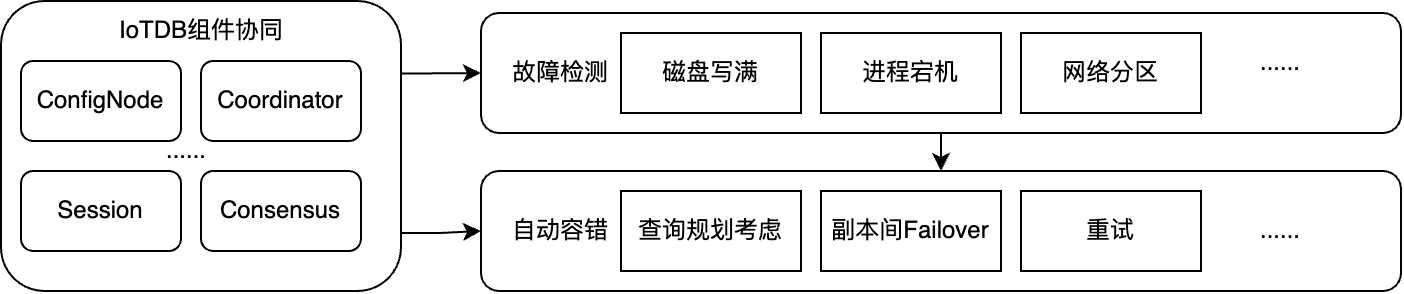
\includegraphics[width=0.99\linewidth]{1-overview-arch.png}
  \caption{IoTDB整体的高可用框架设计}
  \label{fig:c01-overview-arch}
\end{figure}

2. 为Apache IoTDB实现更完善的高可用和容错能力。完善集群的故障检测能力,使IoTDB能够更早、更准确、更全面地发现集群中发生的各种故障。完善集群的故障恢复和转移能力,无需人工干预即可自动执行故障转移,提升IoTDB分布式系统的韧性,使其能够应对更广泛的故障场景。整体的建设目标如图\ref{fig:c01-overview-arch}所示。


3. 对Apache IoTDB的高可用能力进行全面的测试与验证。本文将设计一系列覆盖各种故障场景的测试用例,包括模拟节点失效、网络分区、磁盘故障等。测试将关注系统的故障检测速度、恢复时间、数据一致性以及对系统整体性能的影响等方面。通过严谨的实验和数据分析,我们将验证所构建的高可用性架构是否能够达到预期的目标。



\section{主要贡献}

本文的贡献主要体现在以下几个方面:

1. 系统地建立了Apache IoTDB的高可用框架,在分析分布式系统中常见的故障种类,分析了故障的共性后,并参考现有的分布式系统中常用的高可用建设、故障检测和容错机制,构建了IoTDB的架构和方法论。



2. 完善了Apache IoTDB的故障检测能力和自动容错和转移能力。
本文构建了更加完善的故障检测机制,能够对磁盘写满、进程故障、网络对称分区、网络非对称分区等故障进行识别,且识别速度更快、识别精度更高。
同时,本文还构建了更加完善的故障容错和转移能力。通过ConfigNode、客户端Session、服务端协调者、服务端共识模块等多个关键组件的协同,使得IoTDB能够在上述情况发生时,通过自动化故障转移机制保证服务的持续运行,提升系统的可用性。


3. 通过大量的测试和实验,证明了该高可用架构能够有效解决现有问题并应对新的挑战,为构建高可靠的分布式系统提供了实践支撑和数据验证。


\section{组织结构}
本文共分为8个章节,每个章节的内容如下:

第1章为引言部分,介绍了工业物联网、时间序列数据、时序数据库、Apache IoTDB、分布式数据库中的高可用性和容错能力等背景,阐述了本文建设更极致、更完善的可用性的研究动机,概括了本文的研究内容和研究贡献,描述了本文的组织结构。

第2章为相关研究综述,重点介绍了学术界对于分布式系统故障、高可用容错相关的研究,以及工业界多个广泛应用的分布式系统如Apache Cassandra、TiDB和OceanBase中的高可用方案的介绍。

第3章介绍了集群的故障检测和发现机制,包括基于ConfigNode Leader和DataNode之间心跳的节点存活探测、基于DataNode和DataNode之间心跳的集群拓扑探测、基于Phi Accrual算法的故障研判机制、基于集群监控的故障发现能力,以及加速故障发现的若干优化。

第4章介绍了集群的故障恢复和容错能力,包括客户端、协调者、共识模块的三层联合容错机制。介绍了共识模块提供的数据副本容错基础,协调者模块利用多副本重试的容错尝试,客户端利用重试解决集群的暂时故障状态或不一致状态的能力,并阐述了故障时期的熔断和降级措施。

第5章介绍了集群对于经典故障场景的容错流程。结合第3章的故障检测和发现机制、第4章的故障恢复和容错机制,IoTDB集群能够抵御例如磁盘写满、进程宕机、网络对称/非对称分区、集群变更时的不一致等问题,并给出每种场景的详细容错流程。

第6章为实验部分。

第7章总结了本文的工作和不足之处,并指出了未来工作的主要方向。